%%%%%%%%%%%%%%%%%%%%%%%%%%%%%%%%%%%%%%%%%
% Journal Article
% LaTeX Template
% Version 1.4 (15/5/16)
%
% This template has been downloaded from:
% http://www.LaTeXTemplates.com
%
% Original author:
% Frits Wenneker (http://www.howtotex.com) with extensive modifications by
% Vel (vel@LaTeXTemplates.com)
%
% License:
% CC BY-NC-SA 3.0 (http://creativecommons.org/licenses/by-nc-sa/3.0/)
%
%%%%%%%%%%%%%%%%%%%%%%%%%%%%%%%%%%%%%%%%%

%----------------------------------------------------------------------------------------
%	PACKAGES AND OTHER DOCUMENT CONFIGURATIONS
%----------------------------------------------------------------------------------------

\documentclass[twoside,twocolumn]{article}

\usepackage{blindtext} % Package to generate dummy text throughout this template 
\usepackage{algorithm}% http://ctan.org/pkg/algorithm
\usepackage{algpseudocode}
\usepackage{amsmath}
\usepackage{graphicx}
\graphicspath{ {/Users/alexandre/Desktop/MEC201}}

\usepackage[sc]{mathpazo} % Use the Palatino font
\usepackage[T1]{fontenc} % Use 8-bit encoding that has 256 glyphs
\linespread{1.05} % Line spacing - Palatino needs more space between lines
\usepackage{microtype} % Slightly tweak font spacing for aesthetics

\usepackage[english]{babel} % Language hyphenation and typographical rules

\usepackage[hmarginratio=1:1,top=32mm,columnsep=20pt]{geometry} % Document margins
\usepackage[hang, small,labelfont=bf,up,textfont=it,up]{caption} % Custom captions under/above floats in tables or figures
\usepackage{booktabs} % Horizontal rules in tables

\usepackage{lettrine} % The lettrine is the first enlarged letter at the beginning of the text

\usepackage{enumitem} % Customized lists
\setlist[itemize]{noitemsep} % Make itemize lists more compact

\usepackage{abstract} % Allows abstract customization
\renewcommand{\abstractnamefont}{\normalfont\bfseries} % Set the "Abstract" text to bold
\renewcommand{\abstracttextfont}{\normalfont\small\itshape} % Set the abstract itself to small italic text

\usepackage{titlesec} % Allows customization of titles
\renewcommand\thesection{\Roman{section}} % Roman numerals for the sections
\renewcommand\thesubsection{\roman{subsection}} % roman numerals for subsections
\titleformat{\section}[block]{\large\scshape\centering}{\thesection.}{1em}{} % Change the look of the section titles
\titleformat{\subsection}[block]{\large}{\thesubsection.}{1em}{} % Change the look of the section titles

\usepackage{fancyhdr} % Headers and footers
\pagestyle{fancy} % All pages have headers and footers
\fancyhead{} % Blank out the default header
\fancyfoot{} % Blank out the default footer
\fancyhead[C]{Alexandre Chong - Homework 5 - ME 233} % Custom header text
\fancyfoot[RO,LE]{\thepage} % Custom footer text

\usepackage{titling} % Customizing the title section

\usepackage{hyperref} % For hyperlinks in the PDF

%----------------------------------------------------------------------------------------
%	TITLE SECTION
%----------------------------------------------------------------------------------------

\setlength{\droptitle}{-4\baselineskip} % Move the title up

\pretitle{\begin{center}\Huge\bfseries} % Article title formatting
\posttitle{\end{center}} % Article title closing formatting
\title{ME 233 - Homework 5: State Estimation - Particle Filter} % Article title
\author{%
\textsc{Alexandre Chong} \\[1ex] % Your name
\normalsize University of California, Berkeley \\ % Your institution
\normalsize \href{mailto:alex.chong@berkeley.edu}{alex.chong@bekeley.edu} % Your email address
}
\date{\today} % Leave empty to omit a date

%----------------------------------------------------------------------------------------

\begin{document}

% Print the title
\maketitle

%----------------------------------------------------------------------------------------
%	ARTICLE CONTENTS
%----------------------------------------------------------------------------------------

\section{Introduction}

\lettrine[nindent=0em,lines=3]{T}o estimate the position and heading of this bicycle. I decided to use a particle filter.

The following system states and variables will be approximated through the particle filter.
\begin{itemize}
\item $x$ - position of bike in x-y plane
\item $y$ - position of bike in x-y plane
\item $\theta$ - heading of bike in x-y plane
\item $R$ - radius of bike wheel
\item $B$ - base length of bike
\end{itemize}
%------------------------------------------------
\section{Modeling}

\subsection{GPS Characterization}
Looking at the data from run 0. Where the bike is not moving. It can be seen that the GPS measurements are zero mean and approximately normally distributed.

\begin{table}[h!]
\centering
\caption{GPS True Values}
\label{table:alg1}
\begin{tabular}{rrr}
\hline
$X$ & $Y$ & $\theta$ \\ [0.5ex] 
\hline
$0.20644$ & $1.2318$ & $1.0909$\\
\hline
\end{tabular}
\end{table}

\begin{table}[h!]
\centering
\caption{GPS Calibration}
\label{table:alg1}
\begin{tabular}{rrrr}
\hline
$\bar{X}$ & $\bar{Y}$ & $Var(X)$ & $Var(Y)$\\ [0.5ex] 
\hline
$0.002$ & $0.04$ & $1.088$ & $2.984$\\
\hline
\end{tabular}
\end{table}

\begin{figure}[h]
\caption{Statistics of GPS Calibration Data}
\label{fig:hist}
\centering
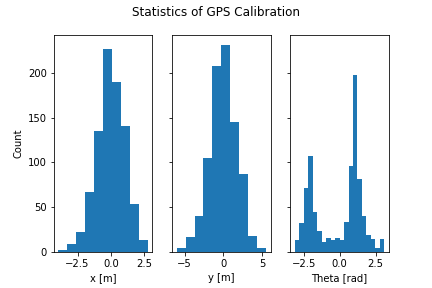
\includegraphics[width=0.5\textwidth]{hist.png}
\end{figure}

The $\theta$ values from the GPS measurement data are bimodally distributed with the maximum likelihood centered around the true value (Figure \ref{fig:hist}).

\subsection{System Dynamics}
The following equations describe how the state of the bike evolves with time. Note that the bike's actual linear speed, velocity, and steering angle readings are modeled as not being exactly as reported.

\begin{center}
$\hat{\omega} = \omega + \nu_\omega$

$\hat{v} =  \hat{\omega} R N + \nu_v$

$\hat{\gamma} = \gamma + \nu_\gamma$

$x[k+1] = x[k] + \Delta t \hat{v}cos(\theta)$

$y[k+1] = y[k]  + \Delta t \hat{v} sin(\theta)$

$\theta[k+1] = \theta[k] + \Delta t \frac{\hat{v}}{B} tan(\hat{\gamma})$
\end{center}

\begin{itemize}
\item $N$ - gear ratio
\item $\gamma$ - reported steering input
\item $\omega$ - reported pedal speed
\item $\Delta t$ - time step
\end{itemize}

\subsection{Noise Modeling}

The following distributions were used to inject process noise into the particle filter.
$N(0,\omega_p)$ represents a zero-mean normally distributed random variable with $\omega_p$ standard deviation.

\begin{center}
$\nu_v \sim  N(0, v_p)$

$\nu_\omega \sim N(0, \omega_p)$

$\nu_\gamma \sim N(0, \gamma_p) $
\end{center}

\begin{table}[h!]
\centering
\caption{Noise Parameters}
\label{table:noise}
\begin{tabular}{rrr}
\hline
$v_p$ & $\omega_p$ & $\gamma_p$ \\ [0.5ex] 
\hline
$0.05$ & $0.10$ & $0.05$\\
\hline
\end{tabular}
\end{table}

The noise parameters in Table \ref{table:noise} are guesses as to what the actual noise looks like.

\subsection{Particle Filter}

\subsubsection{Initialization}
The particle filter is initialized as follows:

\begin{table}[h!]
\centering
\caption{Initial State - Normally Distributed}
\label{table:noise}
\begin{tabular}{rrrr}
\hline
 &$X$ & $Y$ & $\theta$ \\ [0.5ex] 
\hline
mean & $0$ & $0$ & $\frac{\pi}{4}$\\
std & $2.0$ & $2.0$ & $\frac{\pi}{4}$\\
\hline
\end{tabular}
\end{table}

\begin{table}[h!]
\centering
\caption{System Parameters - Uniformly Distributed}
\label{table:noise}
\begin{tabular}{rrr}
\hline
 &$R$ & $B$\\ [0.5ex] 
\hline
min & $0.425 - 0.425\times0.05$ & $0.8 - 0.8 \times 0.1$\\
max & $0.425 + 0.425\times0.05$ & $0.8 + 0.8 \times 0.1$\\
\hline
\end{tabular}
\end{table}

\subsubsection{Procedure}

After initialization, the particles are propagated though the noisy system model at every time step. At time steps with measurements the conditional probability density is created using the normally distributed GPS model.

The weighted particles are then resampled and roughening is added. Roughening is only added to the x, y, and $\theta$ states as R and B are constant with time.

\subsubsection{Roughening}

Roughening is normally distributed and zero mean, it uses the following standard deviation:

\begin{center}
$\sigma_x = K |x_{max} - x_{min}| N^{-\frac{1}{d}}$

$\sigma_y = K |y_{max} - y_{min}| N^{-\frac{1}{d}}$

$\sigma_\theta = K |\Delta\theta_{max}| N^{-\frac{1}{d}}$
\end{center}

In this case $K = 0.1, N = 10000, d = 3$

\section{Design Decisions and Justifications}

The particle filter was chosen for the following reasons:
\begin{itemize}
\item Code does not have to run in real time
\item PF with "many" particles will out-perform the other techniques we learned in class for nonlinear systems (e.g. UKF, EKF)
\end{itemize}

Roughening was not added to system parameters R and B as they do not change with time.

Noise was normally distributed as there is no other reason to suspect otherwise.

The variance for roughening was picked based on the suggestion presented in class.

N = 10,000 was selected as it seemed "large" enough. Was unsure if 15 second constraint was to execute one run or all the runs.

\section{Evaluation and Discussion}

\begin{figure}[h]
\caption{Run 1: Measurements and State Estimate}
\label{fig:top}
\centering
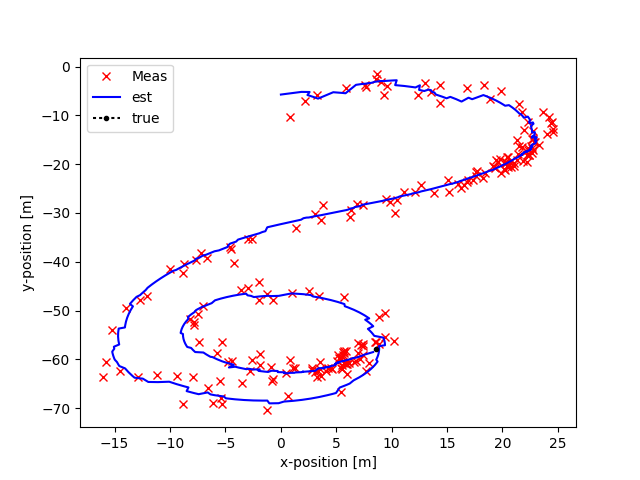
\includegraphics[width=0.5\textwidth]{topview.png}
\end{figure}

\begin{figure}[h]
\caption{Run 1: Measurements, State Estimate, Inputs}
\label{fig:time}
\centering
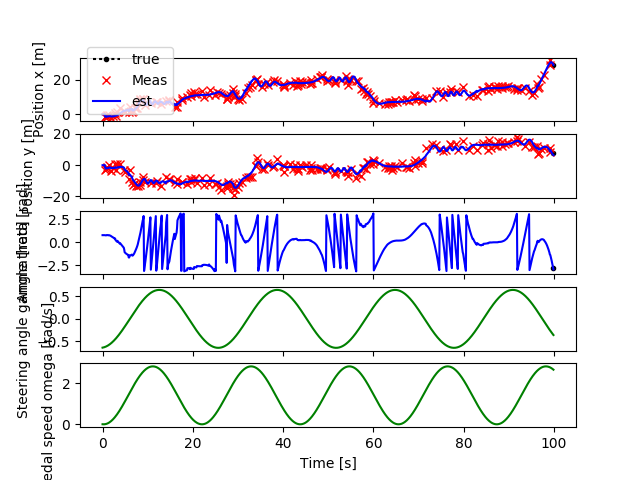
\includegraphics[width=0.5\textwidth]{timeseries.png}
\end{figure}

The particle filter does reasonably well at going through all the points (Figure \ref{fig:top}) and maintaining a relatively smooth trajectory that matches the given inputs (Figure \ref{fig:time}).

Estimation could be greatly improved with a more lower variance gps sensor, a higher gps sample rate, and/or an additional sensor to help provide heading information (e.g. compass).

%----------------------------------------------------------------------------------------

\end{document}
